\section{Markov Chain Monte Carlo simulations}

\todo[color = yellow, inline]{Til Aurora. Jeg tenker at det er kjekt å se hvem som har lagt inn kommentarer i teksten, så hvis du bruker en annen farge enn oransje, så er det lett å skille på hvem sine kommentarer det er. Fargen kan endres til noe annet enn gul om du vil.}
\todo[color = yellow]{om du ikke vil ha kommentaren inline}

In this problem, we are looking at a well known data set of time intervals between successive coal-mining disasters in the UK involving ten or more killed. We will adopt a Bayesian model to analyse the data and implement both a single site and a block Metropolitan-Hastings algorithm to find the underlying distribution of the parameters involved in the model. To to so we will find the posterior distribution of the underlying model parameters and the full conditional for each of the model parameters. 

\subsection{Data exploration}
To get a greater understanding of the data set, the data set is plotted. This can be seen in figure \ref{fig:cumul_plot}, where we have plotted the year along the x-axis and the cumulative number of disasters along the y-axis. 

\begin{figure}[h]
    \centering
    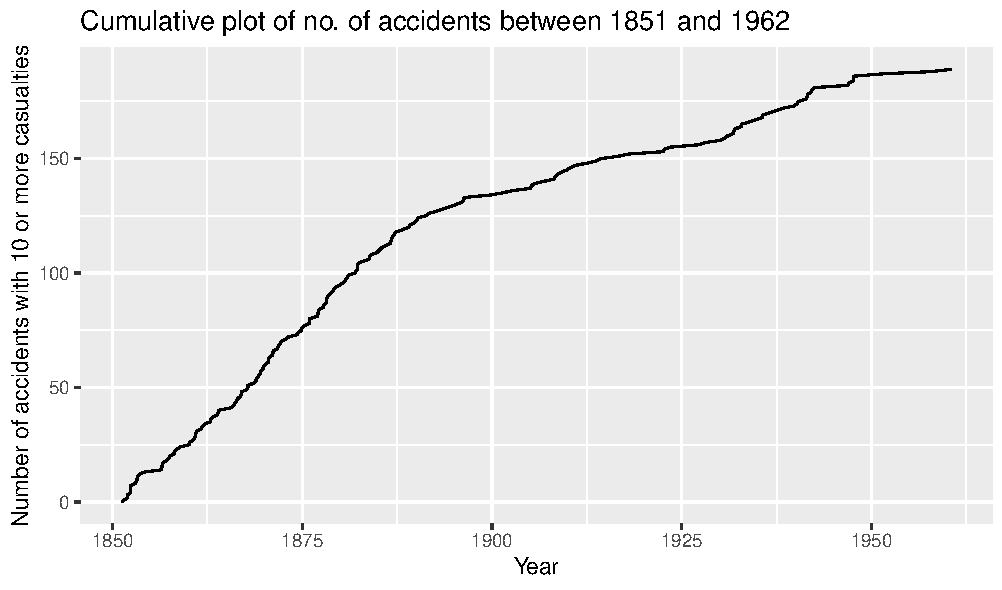
\includegraphics[width = \textwidth]{Images/cumulative_plot_data.pdf}
    \caption{Cumulative plot of coal-mining disasters in the UK occurring between 1851 and 1962.}
    \label{fig:cumul_plot}
\end{figure}

We can instantly see that the incline of the graf is different at the begining and the end of the period. It loks like this shift happens some time between 1885 and 1900. 


\subsection{Posterior distribution of underlying model parameters} \label{posterior}
\todo[color = yellow]{Litt pirk her men når tenksten er såpass lik oppgaveteksten synes jeg der er ryddig å på en måte referere til oppgaven så det kommer tydelig fram at vi ikke har funnet det på selv. Jeg skrev det også om bittelitt}

As proposed in the exercise set we are adopting a hierarchical Bayesian model to analyse the data set. We assume that the coal-mining disasters follow a inhomogeneous Poisson process with intensity function $\lambda(t)$. We assume $\lambda(t)$ to be piecewise constant with $n$ breakpoints. The start and endpoints are denoted by $t_0$ and $t_{n+1}$ for the data set and let $t_k; k = 0,...,n$ denote the break points of the intensity function. In our case we only have one break point. This means,  
\todo{Trenger jeg ha med all denne forklaringen, eller er det nok å si at n = 1 litt tidligere?} 
\todo[color = yellow]{Forklaringen er fin men vi kan gjøre herifra og ut med våre parametre :) }

\begin{align}
    \lambda_0 = \textbf{for } t \in [t_0,t_{1}]) \text{ and }\\
    \lambda_1 = \textbf{for } t \in [t_1, t_2].
\end{align}

The likelihood function for the observed data is given by,

\begin{align}
    f(x|t_1,\lambda_1,\lambda_2) 
    = exp \Big( - \sum_{k = 0}^1 \lambda_k (t_{k-1} - t_k) \prod_{k = 0}^1 \lambda_k^{y_k} \Big), 
\end{align}
where $x$ is the observed data and $y_k$ is the number of observed disasters in the period $t_k$ to $t_{k+1}$. 

We assume $t_1$ to be apriori uniformly distributed on $[t_0, t_2]$, and $\lambda_0, \lambda_1$ to be apriori independent of $t_1$ and of each other. We also assume $\lambda_0,\lambda_1$ to have the gamma prior distribution with $\alpha = 2$ and scale parameter $\beta$. Thus, we have 

\begin{align}
    \pi(\lambda_i | \beta) = \frac{1}{\beta^2}\lambda_i e^{-\frac{\lambda_i}{\beta}} \textbf{ for } \lambda_i \geq 0.
\end{align}

The hyper parameter $\beta$ follows the following improper distribution,

\begin{align}
    \pi (\beta) \propto \frac{exp\{ -\frac{1}{\beta} \} }{\beta} \textbf{ for } \beta > 0.
\end{align}

In total this gives us the following model parameters, $\boldsymbol{\theta} = (t_1, \lambda_0, \lambda_1, \beta)$. 
To find an expression for the posterior distribution of $\boldsymbol{\theta}$ given $x$, $f(\boldsymbol{\theta}|x)$, we use Bayes' theorem, and find that 
\todo{forklar mer hvordan vi kommer fram til dette?}
\todo[color = yellow]{la til mellomsteget. Det er ikke egentlig noe mer og forklare her det er sånn Bayes formula er definert :) }
\begin{align}
    f(\theta|x) = \frac{f(x|\theta) \pi(\theta)}{f(x)} \propto f(x|\theta) \pi(\theta) .
\end{align}
The likelihood $f(x | \boldsymbol{\theta})$ is given above, $\pi(\boldsymbol{\theta})$ can be computed knowing $t_1, \lambda_0$ and $\lambda_1$ are all independent. In total this means,

\begin{align}
    \pi(\boldsymbol{\theta}) 
    = \pi(t_1, \lambda_0, \lambda_1, \beta) \nonumber \\
    = \pi(t_1, \lambda_0, \lambda_1 | \beta) \cdot \pi(\beta) \nonumber \\
    = \pi(t_1) \cdot \pi(\lambda_0|\beta) \cdot \pi(\lambda_1|\beta) \cdot \pi(\beta).
\end{align}

Using this and the given likelihood, we find the posterior distribution for $f(\boldsymbol{\theta}|x)$

\begin{align} \label{eq:post}
    f(\boldsymbol{\theta}|x) \propto exp \Big( - \sum_{k = 0}^1 \lambda_k (t_{k+1} - t_k) \Big)\cdot \prod_{k = 0}^1 \lambda_k^{y_k} \cdot \frac{1}{t_2-t_0} 
    \Big( \frac{1}{\beta^2} \lambda_0 \cdot
    exp \Big({-\frac{\lambda_0}{\beta}} \Big)  \Big) \nonumber \\ 
    \cdot \Big( \frac{1}{\beta^2} \lambda_1 \cdot exp \Big({-\frac{\lambda_1}{\beta}} \Big) \Big) \cdot exp \Big( -\frac{1}{\beta} \Big)/\beta \nonumber \\
    \propto   \frac{1}{\beta^5} \cdot \lambda_0^{y_0 + 1} \cdot \lambda_1^{y_1 + 1} \cdot exp \Big( -\frac{1}{\beta}(\lambda_0 + \lambda_1 + 1) - \lambda_0(t_1-t_0) - \lambda_1(t_2-t_1) \Big)
\end{align}




%%%%%%%%%%%%%%%%%%%%%%%%%%%%%%%%%%%%%%%%%%%%%%%%%%%%%%%%%%%%%%%%%%%%%%%%%%%%%%%%%%%%%%%%%%%%%%%%%%%%%%%%%%%%%%%%%%%%%%%%%%%%%%%
\subsection{Full conditional distribution for the model parameters} \label{full_cond}

To find the full conditional for each of the elements in $\boldsymbol{\theta}$, we use the expression for the posterior distribution given in \eqref{eq:post}. When we are looking at the full conditional for one of the elements in $\theta$ gven all the others, the other parameters can be viewed as constants. This means what we can overlook them in our proportional model, and we get that the full conditional for $t_1$ is

\begin{align}
    f(t_1 | \lambda_0, \lambda_1, \beta, x) \propto 
    \lambda_0^{y_0 + 1} \lambda_1^{y_1 + 1} \cdot exp \Big( -\lambda_0(t_1 - t_0) - \lambda_1 (t_2 - t_1) \Big) \nonumber \\
    \propto  \lambda_0^{y_0 + 1} \lambda_1^{y_1 + 1} \cdot exp \Big( -(\lambda_0 - \lambda_1)t_1 \Big).
\end{align}

We do not recognize the expression for the full conditional of $t_1$ as belonging to a named distribution. 

The full conditional for $\lambda_0$ and $\lambda_1$ can also be found by using the posterior distribution given in \eqref{eq:post}. Thus, 

\begin{align}
    f(\lambda_0 | \lambda_1, t_1, \beta, x) \propto
    \lambda_0^{y_0 + 1}\cdot exp \Big( -\frac{1}{\beta} \lambda_0 - (t_1 - t_0)\lambda_0 \Big) 
    \nonumber \\
    \propto  \lambda_0^{y_0 + 1} \cdot exp \Big( - \lambda_0 (\frac{1}{\beta} + t_1 - t_0) \Big),
     \\
    f(\lambda_1 | \lambda_0, t_1, \beta, x) \propto
    \lambda_1^{y_1 + 1}\cdot exp \Big( -\frac{1}{\beta} \lambda_1 - (t_2 - t_1)\lambda_1 \Big) \nonumber \\
    \propto  \lambda_1^{y_1 + 1} \cdot exp \Big( - \lambda_1 (\frac{1}{\beta} + t_2 - t_1) \Big),
\end{align}
and we see that the full conditional for $\lambda_0$ and the full conditional for $\lambda_1$ are both gamma distributed with rate, $\alpha$, and scale, $\beta$, parameters respectivly $\alpha_0 = y_0 + 2$, $\beta_0 = \frac{1}{\frac{1}{\beta} + t_1 - t_0}$, $\alpha_1 = y_1 + 2$, $\beta_1 = \frac{1}{\frac{1}{\beta} + t_2 - t_1}$. 



For the last parameter $\beta$, the full conditional is given by,

\begin{align}
    f(\beta | \lambda_0, \lambda_1, t_1, x) \propto 
    \frac{1}{\beta^5} \cdot exp \Big( -\frac{1}{\beta}(\lambda_0 + \lambda_1 + 1) \Big),
\end{align}

and we also recognize this as belonging to a gamma distribution with rate parameter $\alpha_{\beta} = 6$ and scale parameter $\beta_{\beta} = \frac{1}{\lambda_0 + \lambda_1 + 1} $. 

\subsection{Single site MCMC algorithm}

We have defined and implemented a single site MCMC algorithm for $f(\theta |x)$. $f(\theta|x)$ is the target distribution we want to sample from seen in equation \ref{eq:post}.  As the full conditionals of $\beta^i, \lambda_0^i$ and $\lambda_1^i$ belong to known distributions, we can use Gibbs sampling to draw directly from the full conditionals for these parameters. For $t_1$ however, this is not possible.
To find $t_1$, we use the Metropolis-Hastings step with a random walk of order one. This means we propose a new value for $t_1$ which we from now on will call $t$ from the normal distribution with the previous $t$ value as mean and a tuning parameter $\sigma$ as variance. 

\todo[color = yellow]{Her var det noe som ikke ble helt riktig. Det som står nå er rett det som er kommentert ut er ikke helt rett}
% We draw an initial state for $t$ and then propose a new state $t_{new}$ from $Q(t_1|x)$ using a random walk step, where $Q(t_1|x)$ is our proposal distribution. We have chosen our random walk step to be normally distributed with mean $t_{old}$ and standard deviation $\sigma$.

We then compute the acceptance probability for $t_{new}$

\begin{align}
    \alpha(t_{new}|x) = min \Big( 1, \frac{f(t_{new}| \lambda_0, \lambda_1, \beta, x)}{f(t_{old}| \lambda_0, \lambda_1, \beta, x)} \Big) \nonumber \\ 
    = min \Big( \frac{\lambda_0^{y_0 + 1} \cdot \lambda_1^{y_1 + 1} exp(-(\lambda_0 - \lambda_1)t_{new})}{\lambda_0^{y_0 + 1} \cdot \lambda_1^{y_1 + 1} exp(-(\lambda_0 - \lambda_1)t_{old})} \Big) \nonumber \\
    = min \Big( 1, \frac{exp(-(\lambda_0 - \lambda_1)t_{new})}{exp(-(\lambda_0 - \lambda_1)t_{old})} \Big)
\end{align}

and accept or reject the proposed $t$. We note that since the proposal density is a random walk the proposal ration which usually is a part of the acceptance probability cancels out. 

All of this gives us the following algorithm, 

%input code lines here. 
\lstinputlisting[language=R, firstline=3, lastline=57]{Code/MH_singel.R}

\todo{Bør jeg gå mer i detalj om acceptance/rejection her?}



\subsection{Burn-in and mixing period of the algorithm}

To evaluate the burn-in period of the algorithm, we have plotted the values of $\lambda_0, \lambda_1, t_1$ and $\beta$ for $n$ iterations of our MCMC algorithm. This is seen in figure \ref{fig:burnin_singleMH}. 

\todo[color = yellow]{Husk å skrive hva vi har brukt som initialverdier og verdien til sigma}

\begin{figure}[h]
    \centering
    \begin{subfigure}[b]{0.49\textwidth}
        \centering
        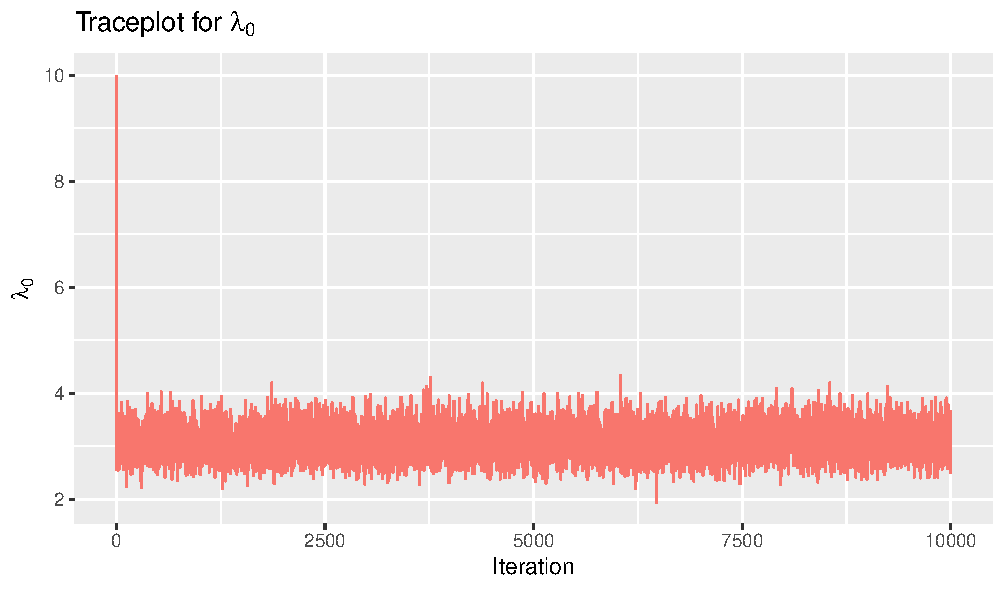
\includegraphics[width = \textwidth]{Images/sim_lambda0.pdf}
        \caption{$\lambda_0$}
        \label{fig:burnin_lam0}
    \end{subfigure}
    \begin{subfigure}[b]{0.49\textwidth}
        \centering
        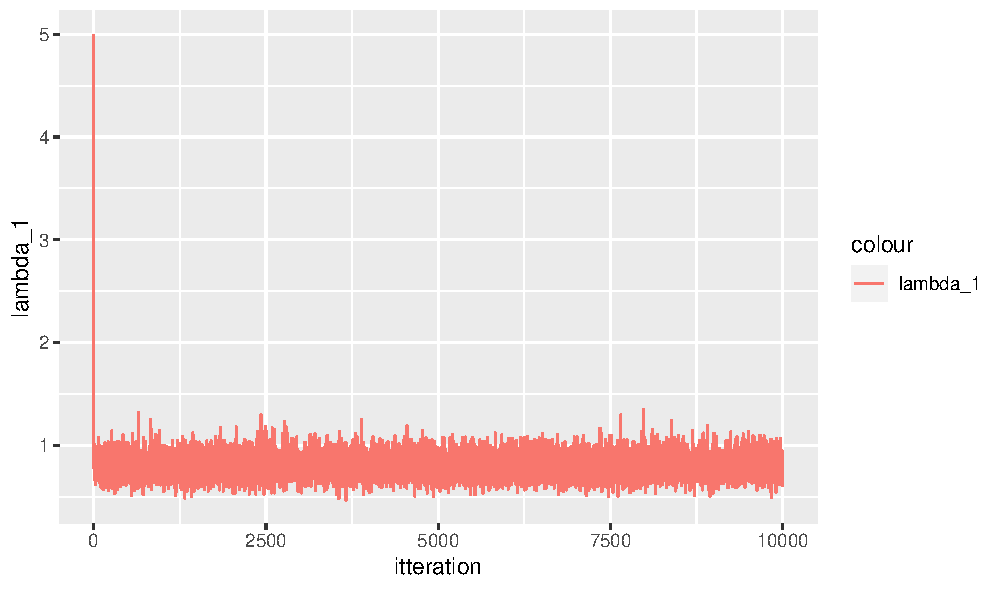
\includegraphics[width = \textwidth]{Images/sim_lambda1.pdf}
        \caption{$\lambda_1$}
        \label{fig:burnin_lam1}
    \end{subfigure}
    \begin{subfigure}[b]{0.49\textwidth}
        \centering
        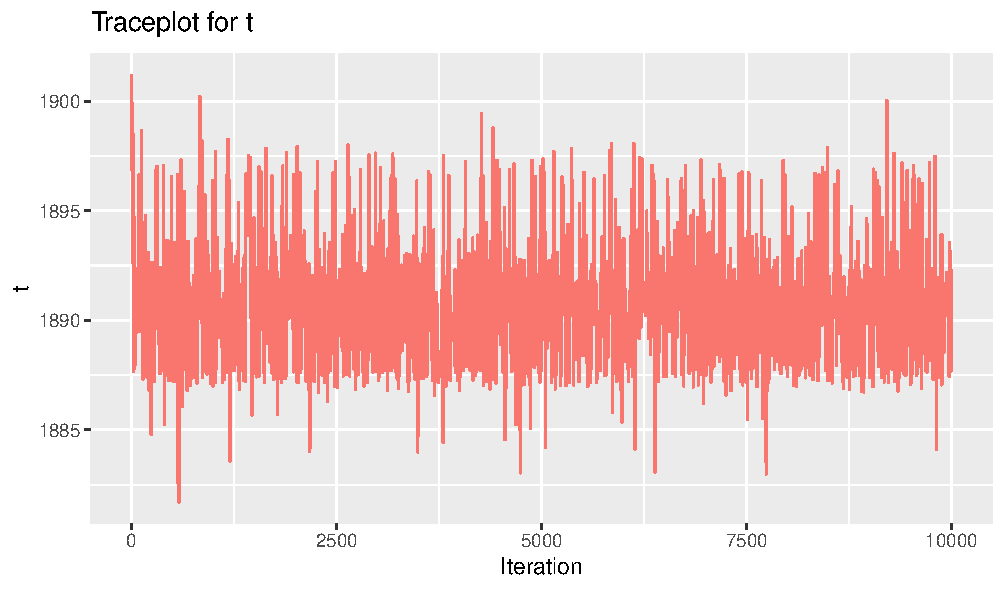
\includegraphics[width = \textwidth]{Images/sim_t.pdf}
        \caption{$t_1$}
        \label{fig:burnin_t}
    \end{subfigure}
    \begin{subfigure}[b]{0.49\textwidth}
        \centering
        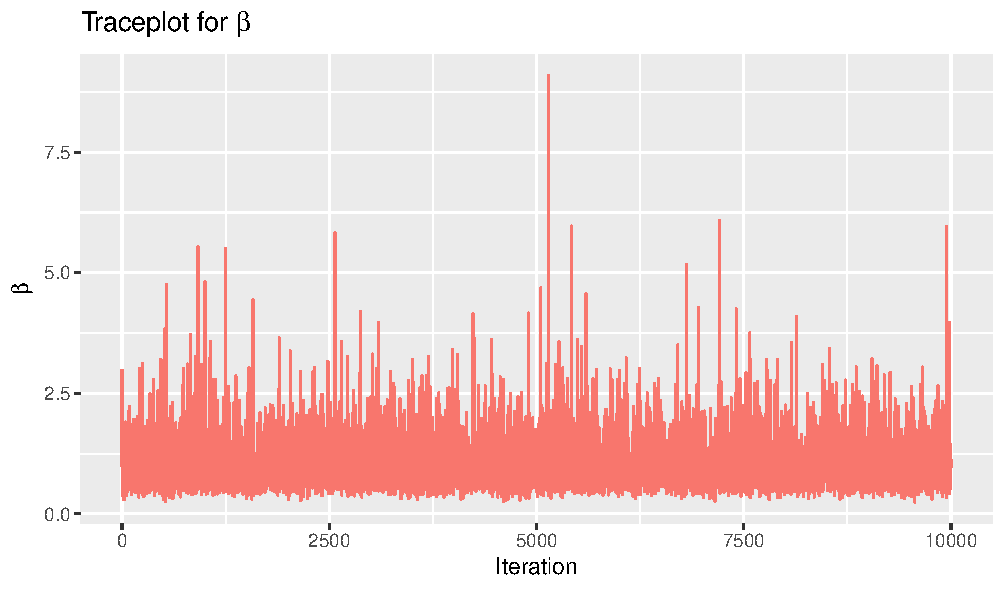
\includegraphics[width = \textwidth]{Images/sim_beta.pdf}
        \caption{$\beta$}
        \label{fig:burnin_beta}
    \end{subfigure}
    \caption{The value of $\lambda_0, \lambda_1, t_1$ and $\beta$ plotted for $n = 10000$ iterations of the MCMC algorithm.}
    \label{fig:burnin_singleMH}
    \todo[color = yellow]{Legg in initialverdier og verdien til sigma her også}
\end{figure}

We plotted the parameters separately so they are easier to evaluate. We need to choose a burn-in period for the algorithm equal to the longest burn-in period amongst the parameters. 
In figure \ref{fig:burnin_lam0} and \ref{fig:burnin_lam1}, we see that the simulations stabilize very quickly, and there is a very small burn-in period for these parameters. 
\todo[inline]{burn-in for beta. Den er ikke helt stabil}
\todo[inline]{Burn-in for t. Ikke helt stabil. Ta med plott fra forskjellige ekstremverdier av t, of forklar hvordan disse ser ut..}
For the parameter $\beta$, we see that the samples fluctuate, but the mean and variance of the simulations does not seem to change. For the $t_1$-parameter however, we see that the mean slightly changes when the number of iterations increase. This means that we should investigate the burn-in period of this parameter more closely. We do this by running the algorithm for a number of different $n$. 

% In figure \ref{fig:sim_t_big_n}, we see the simulations of $t_1$ with $n = 50000$ and $n = 100000$ samples. 

% \begin{figure}[h]
%     \centering
%     \begin{subfigure}[b]{0.49\textwidth}
%         \centering
%         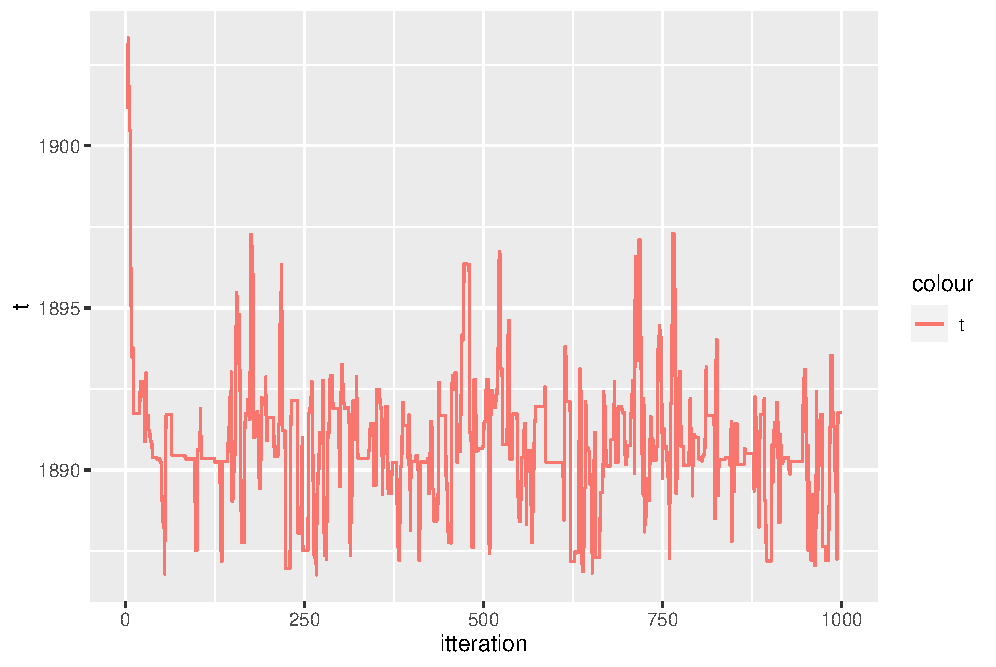
\includegraphics[width = \textwidth]{Images/sim_t_1000.pdf}
%         \caption{$n =1000 $}
%         \label{fig:}
%     \end{subfigure}
%     \begin{subfigure}[b]{0.49\textwidth}
%         \centering
%         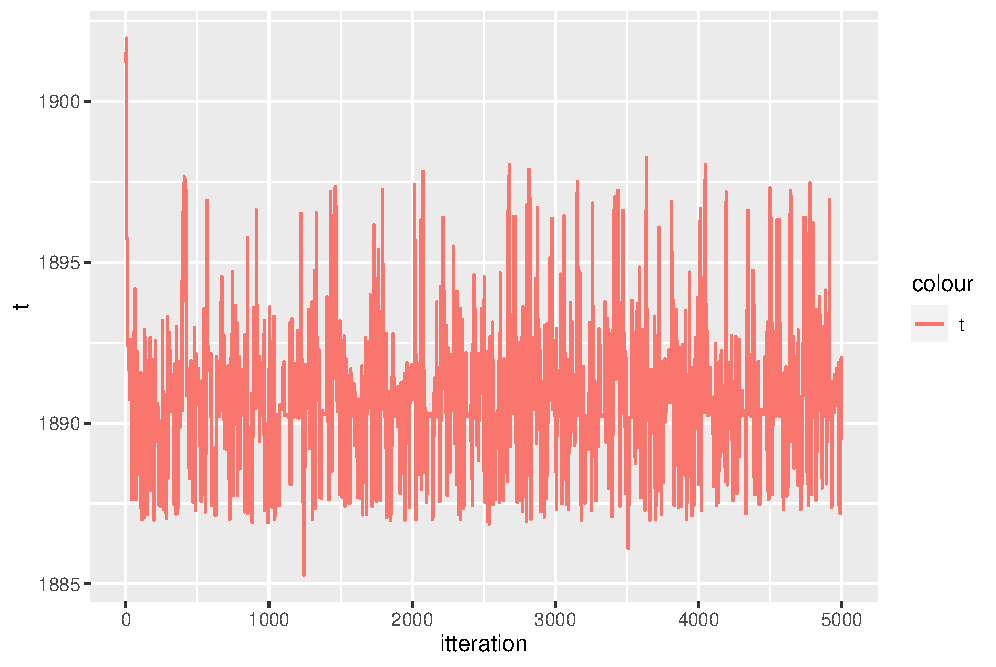
\includegraphics[width = \textwidth]{Images/sim_t_5000.pdf}
%         \caption{$n = 5000 $}
%         \label{fig:}
%     \end{subfigure}
%     \begin{subfigure}[b]{0.49\textwidth}
%         \centering
%         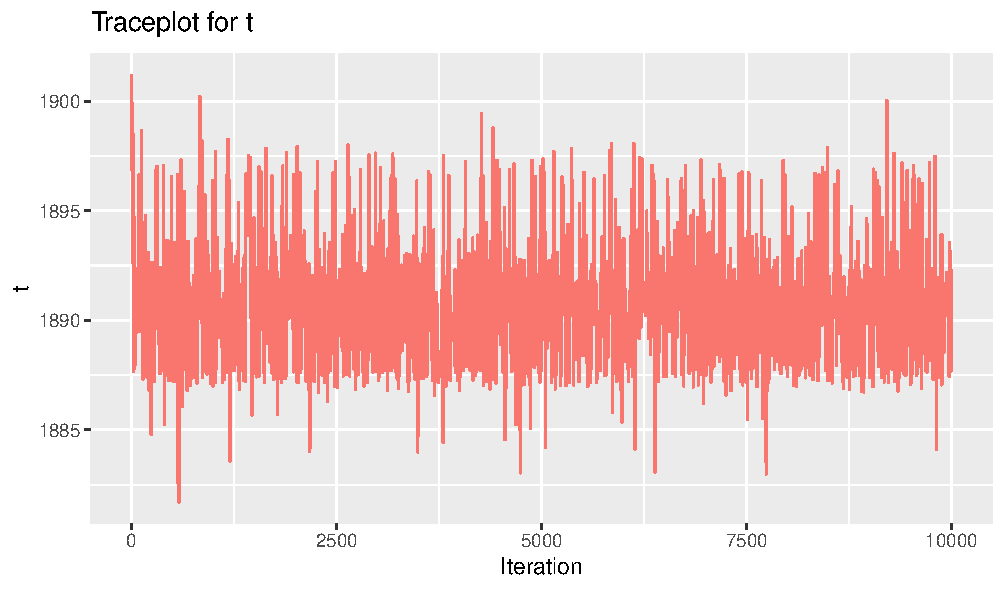
\includegraphics[width = \textwidth]{Images/sim_t.pdf}
%         \caption{$n = 10000$ }
%         \label{fig:}
%     \end{subfigure}
%     \begin{subfigure}[b]{0.49\textwidth}
%         \centering
%         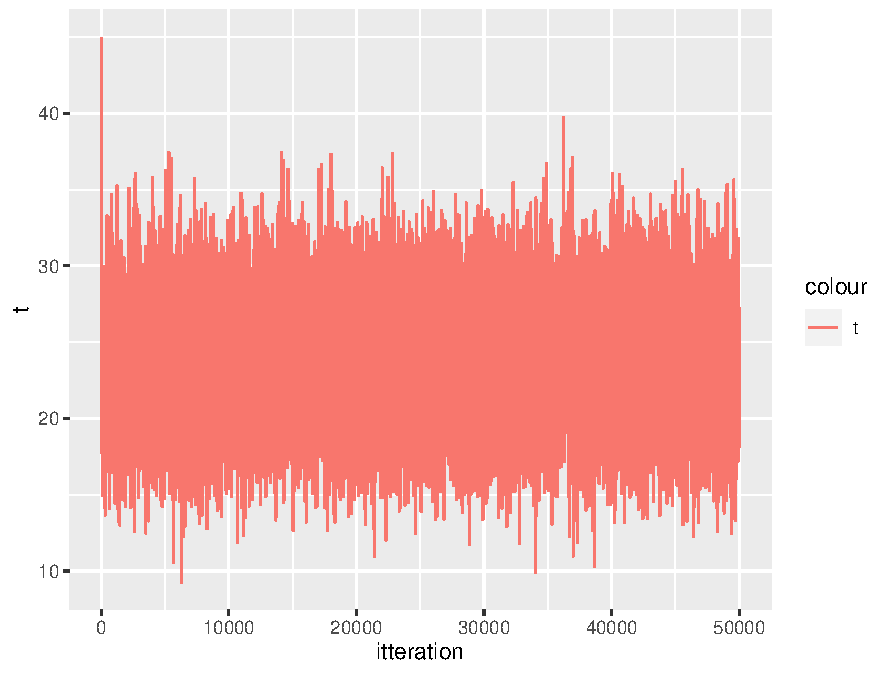
\includegraphics[width = \textwidth]{Images/sim_t_50000.pdf}
%         \caption{$n =  50000$}
%         \label{fig:}
%     \end{subfigure}
%     \caption{Simulations of $t_1$ with $n = 1000, 5000, 10000$ and $n=50000$ samples. }
%     \label{fig:sim_t_big_n}
% \end{figure}

% We see that the simulations of $t_1$ in figure \ref{fig:sim_t_big_n} 

\todo[inline]{separate into two areas and calculate the statistics for the areas to evaluate if we have chosen an okay estimate for the burn-in period.}


%mixing
\todo[color = yellow]{Dette er forsåvidt rett men ha også med et plott med to forskjellig kjeder og se hvordan de mikser}
To evaluate the mixing properties of our algorithm, we first plot the autocorrelation function for our parameter $t_1$ after the initial burn-in period, which we have set to be $b = *???$ iterations. The autocorrelation plot is shown in figure \ref{fig:acf_t}. From the plot we see that the correlation decreases between the samples as the distance increases, and after $lag = 20$, there is no significant autocorrelation between the drawn samples. This indicates that the mixing is not slow. 

\begin{figure}[h]
    \centering
    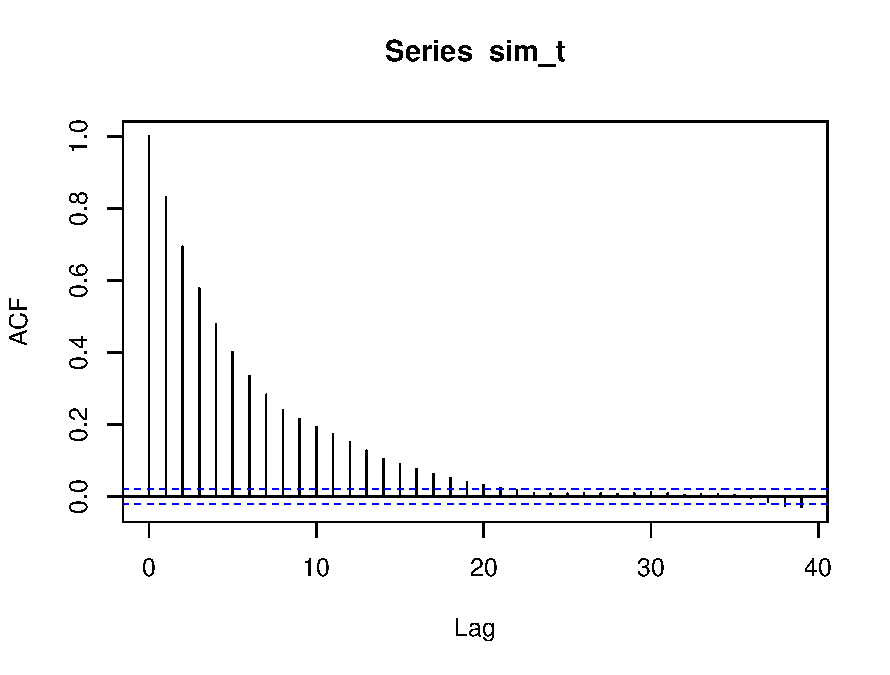
\includegraphics{Images/acf_t_10000.pdf}
    \caption{Autocorrelation function of $t_1$ for different $lag$. }
    \label{fig:acf_t}
\end{figure}

\todo[color = yellow]{Her skal det være convergense property. Det er jo verdien som det convergeres mot som må være reasonable ift original datasettet}
To investigate the mixing property further, we can 
\todo[inline]{Use the plot generated in 1 to simulate whether the simulated values are reasonable.}

\subsection{The tuning parameter and how it influences the burn-in and mixing of the simulated Markov Chain}

We have implemented our Markov Chain Monte Carlo algorithm with a tuning parameter $\sigma$. The tuning parameter is the variance for our proposal distribution $Q()$. $\lambda_0, \lambda_1$ and $\beta$ are drawn from known distributions, so the tuning parameter will not affect these samples that much. For our parameter $t$ however, the tuning parameter will change the acceptance rate of the algorithm. By using a small tuning parameter $\sigma$, the new proposal $t_{new}$ will be similar to the old value $t_{old}$ and the mixing will be slow. When increasing the tuning parameter, the variance in the proposal distribution is increased, and $t_{new}$ will vary more from $t_{old}$. This means that correlation between the samples decreases and the mixing increases. We cant to adjust the tuning parameter such that we get enough mixing for the algorithm to take large enough steps to explore the target density efficiently, but not so large that the acceptance rate becomes too low. We are looking for an acceptance rate of $20 - 50\%$. In figure \ref{"Set in plots with different values of sigma t"} we can see how the tuning parameter $\sigma$ affects the simulated samples of $t$.  Here we see that with $\sigma = 0.2$, the steps taken are very small. This leads to a slow exploration of the target density, and we see that $n = 10000$ iterations are far too few for the algorithm to converge. This again leads to a very large burn-in period. For $\sigma = 3$, we see that the there is enough mixing for the samples to quickly converge, and the burn-in period thus become small. If we use a very large tuning parameter, for instance $\sigma = 30$, the should be little correlation between $t_{new}$ and $t_{old}$. This means that large moves are proposed, but not often accepted. 

%Skriv noe om at stegene aksepteres mindre ofte, men fortsatt ganske ofte med sigma = 30. Skriv også hvorfor vi ikke kan ha hæyere sigma. Fordi det blir maskinelt 0 når eksponentene i e i uttrykket blir for store?

\todo[inline]{Error om vi bruker for stor sigma. Klarer ikke kjøre med f.eks sigma = 50. Se på grunner til dette. }
\todo[inline]{legg inn figurer, sigma = 0.2, sigma = 3, Sigma = 30}


\subsection{Implementing a block Metropolis-Hastings algorithm}

To improve the performance of our Metropolis-Hastings algorithm, we can perform blocking of the parameters. This means that not all parameters in $\theta$ are treated individually. Grouping together certain parameters in $\theta$ may be useful when they are correlated. We will then compute the acceptance probability, and either update all parameters within the block or none of them. We will implement a block Metropolis-Hastings algorithm with two blocks.

%A block Metropolis-Hastings algorithm for $f(\theta|x)$ can be defined as 
%skriv noe om Gibbs sampling?

We alternate between blocking together $t_1, \lambda_0$ and  $ \lambda_1$ and keeping $\beta$ unchanged, and blocking $\beta, \lambda_0$ and $\lambda_1$ together, keeping $t_1$ unchanged.


\subsubsection{Using a block proposal for $(t_1, \lambda_0, \lambda_1)$ keeping $\beta$ unchanged}

\todo[inline]{Introduser og skriv litt om target distribution her}
% Target distribution.Introduser og skriv litt rundt denne. Er den helt rett? 
\begin{align}
    f(t_1, \lambda_0, \lambda_1|\beta, x) = exp \Big( -(t_1-t_0)\lambda_0 -(t_2-t_1)\lambda_1 - \frac{1}{\beta}(\lambda_0 - \lambda_1)\Big) \cdot\lambda_0^{y_0 + 1} \cdot \lambda_1^{y_1 + 1} 
\end{align}

% Proposal distribution. Skriv om RW
We use a random walk proposal density, and the random walk proposal values are generated by firstly generating $\widetilde{t_1}$ from a normal distribution, and then using the value for $\widetilde{t_1}$ when generating ($\widetilde{\lambda_0}$, $\widetilde{\lambda_1}$) from their joint full conditional. This is then used as the proposal function. As we assume $\lambda_0$ and $\lambda_1$ independent, we have that 

\begin{align}
    Q(\widetilde{t_1}, \lambda_0, \lambda_1 |t) = f(\lambda_0| \lambda_1, x, \widetilde{t_1}, \beta)\cdot f(\lambda_1| \lambda_0, x, \widetilde{t_1}, \beta)\cdot f(\widetilde{t_1}| t) \nonumber %\\
    % = \lambda_0^{y_0 + 1} \cdot \lambda_1^{y_1 + 1} \cdot exp \Big(  -\lambda_0(\frac{1}{\beta} + \widetilde{t_1} - t_0) - \lambda_1(\frac{1}{\beta} + t_2 - \widetilde{t_1})  \Big)  \nonumber \\ \cdot \frac{1}{\sqrt{2 \pi}\sigma_t } \cdot exp \Big(  -\frac{1}{2} \frac{(\widetilde{t_1}-t_1)^2}{\sigma_t^2} \Big).
\end{align}
\todo[color = yellow]{Vi trenger ikke skrive ut det fulle uttrukket, det over holder. I tillegg er det som er kommentert ut ikke helt riktig husk at lamdaene også har nye og gamele verdier så nesten ingen ting kanselerer}

For the acceptance probability, we have that

%Acceptance probability
\begin{align}
    \alpha = min \Bigg(1,  \frac{
    f(t_{new}, \lambda_{0_{new}}, \lambda_{1_{new}}|\beta, x)}{f(t_{old}, \lambda_{0_{old}}, \lambda_{1_{old}}|\beta, x)}
    \cdot 
    \frac{Q(t_{old}, \lambda_{0_{old}}, \lambda_{0_{old}} | \beta, x, t_{new})}{Q(t_{new}, \lambda_{0_{new}}, \lambda_{0_{new}} | \beta, x, t_{old})} \Bigg) \\
    = min \Bigg(1, \frac{ exp \Big( -\lambda_0t_{1_{new}} +\lambda_1t_{1_{new}}  \Big)}{ exp \Big( -\lambda_0t_{1_{old}} +\lambda_1t_{1_{old}} \Big)} 
    \cdot \frac{ exp \Big(  -\lambda_0 t_{1_{new}} + \lambda_1 t_{1_{new}}   -\frac{1}{2} \frac{(\widetilde{t}_{1_{new}}-t_{1_{new}})^2}{\sigma_t^2} \Big)}{ exp \Big(  -\lambda_0 t_{1_{old}}  + \lambda_1 t_{1_{old}}  -\frac{1}{2} \frac{(\widetilde{t}_{1_{old}}-t_{1_{old}})^2}{\sigma_t^2} \Big)}   \Bigg).
\end{align}

\todo[inline]{Kansellere enda flere termer i uttrykket?}



\subsubsection{Using a block proposal for $\beta, \lambda_0, \lambda_1$ keeping $t_1$ unchanged}

To generate a block proposal for $\beta, \lambda_0, \lambda_1$ keeping $t_1$ unchanged, we have a target distribution which is 


%Target distribution
%Er dette rett? mangler det en $1/beta$ i flere av eksponentene?
\begin{align}
    f(\beta, \lambda_0, \lambda_1| t_1, x) = 
    \lambda_0^{y_0 + 1} \cdot \lambda_1^{y_1 + 1} \cdot \frac{1}{\beta^5} \cdot exp\Bigg(  -\lambda_0(t_1 - t_2) 
    - \lambda_1 (t_2 - t_1 ) 
    - \frac{1}{\beta} \cdot (\lambda_0 + \lambda_1  + 1) \Bigg). 
\end{align}

%Proposal distribution

Again, we choose to have a random walk as our proposal density. Now, we generate the potential values by first generating $\widetilde{\beta}$ from a normal distribution, this being the random walk, and then and then generating ($\widetilde{\lambda}_0, \widetilde{\lambda}_1$) from their resulting joint conditional using $\widetilde{\beta}$, $f(\lambda_0, \lambda_1|x,t_1,\widetilde{\beta})$. 
We again consider $\lambda_0$ and $\lambda_1$ independent, so the joint conditional is just the full conditionals of each multiplied. We can then find an expression for the proposal function,

\begin{align}
    Q(\widetilde{\beta}, \lambda_0, \lambda_1| \beta) = f(\lambda_0| \lambda_1, x, \widetilde{\beta}, t_1)\cdot f(\lambda_1| \lambda_0, x, \widetilde{\beta}, t_1)\cdot f(\widetilde{\beta}| \beta) \nonumber \\
    = \lambda_0^{y_0 + 1} \cdot \lambda_1^{y_1 + 1} \cdot exp \Big( -\lambda_0(\frac{1}{\widetilde{\beta}} + t_1 - t_0) - \lambda_1(\frac{1}{\widetilde{\beta}} + t_2 - t_1)  \Big)  \nonumber \\ \cdot \frac{1}{\sqrt{2 \pi}\sigma_{\beta} } \cdot exp \Big(  -\frac{1}{2} \frac{(\widetilde{\beta}-\beta)^2}{\sigma_{\beta}^2} \Big).
\end{align}



%Acceptance probability

For the acceptance probability, we then have that 

\begin{align}
    \alpha = min \Bigg(1,  \frac{
    f(\beta_{new}, \lambda_{0_{new}}, \lambda_{1_{new}}|t_1, x)}{f(\beta_{old}, \lambda_{0_{old}}, \lambda_{1_{old}}|t_1, x)}
    \cdot 
    \frac{Q(\beta_{old}, \lambda_{0_{old}}, \lambda_{0_{old}} | t_1, x, \beta_{new})}{Q(t_{new}, \lambda_{0_{new}}, \lambda_{0_{new}} | t_1, x, \beta_{old})} \Bigg) %\\
    % = min \Bigg(1, \frac{ exp \Big( -\lambda_0 \beta_{new} +\lambda_1 \beta_{new}  \Big)}{ exp \Big( -\lambda_0 \beta_{old} +\lambda_1 \beta_{old} \Big)} 
    % \cdot \frac{ exp \Big(  -\lambda_0 \beta_{new} + \lambda_1 \beta_{new}  -\frac{1}{2} \frac{(\widetilde{\beta}_{new}-\beta_{new})^2}{\sigma_{\beta}^2} \Big)}{ exp \Big(  -\lambda_0 \beta_{old}  + \lambda_1 \beta_{old}  -\frac{1}{2} \frac{(\widetilde{\beta}_{old}-\beta_{old})^2}{\sigma_{\beta}^2} \Big)}  \Bigg).
\end{align}

\todo[color = yellow]{Se kommentaren over}


%input the code for the algorithm. Remember to clean the code for all print statements. 
\todo[inline]{sette inn koden for algoritmen}
\todo[inline]{Sette inn og kommentere figurer her. }


\subsection{The block Metropolitan-Hastings algorithm for different values of the tuning parameter}

\begin{comment}

\begin{figure}
    \centering
    \begin{subfigure}
        \includegraphics{}
        \caption{Caption}
        \label{fig:my_label}
    \end{subfigure}
    \begin{subfigure}
        \includegraphics{}
        \caption{Caption}
        \label{fig:my_label}
    \end{subfigure}
    \begin{subfigure}
        \includegraphics{}
        \caption{Caption}
        \label{fig:my_label}
    \end{subfigure}
    \caption{}
    \label{fig:sigma_t}
\end{figure}

\begin{figure}
    \centering
    \begin{subfigure}
        \includegraphics{}
        \caption{Caption}
        \label{fig:my_label}
    \end{subfigure}
    \begin{subfigure}
        \includegraphics{}
        \caption{Caption}
        \label{fig:my_label}
    \end{subfigure}
    \begin{subfigure}
        \includegraphics{}
        \caption{Caption}
        \label{fig:my_label}
    \end{subfigure}
    \caption{}
    \label{fig:sigma_beta}
\end{figure}

\end{comment}


In the block Metropolis-Hastings algorithm, we have two different tuning parameters. One for each of the different block proposals. 
\todo[inline]{Se på koden, klarer ikke å kjøre med stor $\sigma_t$ (f.eks $\sigma_t$ = ), og heller ikke med veldig liten $\sigma_{beta}$ (f.eks $\sigma_{beta}$ = 0.003).}


 In figure \ref{}, we have plotted the parameter $t$ and $\beta$ for three different values of $\sigma_t$. We figure \ref{}, we have plotted the simulation of parameters $t$ and $\beta$ for three different values of $\sigma_{\beta}$. The different block proposals does not run completely independently of each other, as the values proposed in one block is used in the other block if accepted. However, we see in figures \ref{} and \ref{} that changing the tuning parameter for one of the block does not greatly change the mixing or acceptance rate for the other block. We do however see how the.... 
 \todo[inline]{Sett inn plott og kommenter de.}